\chapter{Spectroscopie électronique et photophysique}\label{ch:b3:electronic-spectroscopy}

Sous la lampe ultraviolette d'un bar plongé dans la pénombre, un verre de
tonic luit d'un bleu pâle, fantomatique. La quinine qu'il contient absorbe
la lumière ultraviolette, que l'œil ne voit pas, et en restitue une
partie quelques nanosecondes plus tard sous forme de lumière bleue
visible. Absorption, brève existence dans un état excité, émission à une
longueur d'onde plus grande, énergie qui ne revient pas sous forme de
lumière~: le devenir d'une molécule excitée est une compétition entre
processus dotés de constantes de vitesse, et son spectre est façonné par
les vibrations de la molécule et par les règles de symétrie du
\cref{ch:b3:group-theory-applied}. Ce chapitre étudie les transitions
électroniques et ce qui se passe après elles, domaine appelé
photophysique~; le \cref{ch:b3:photochemistry} y ajoute les cas où la
molécule excitée réagit.

\begin{recall}
Le volume de première année a mesuré l'absorbance avec la loi de
Beer--Lambert, $A =
\varepsilon\ell c$, a défini le coefficient d'absorption molaire, les
chromophores et les systèmes conjugués, et a relié la couleur au maximum
d'absorption. Le volume de deuxième année a nommé les orbitales
frontières HO et BV (HOMO et LUMO). Le \Cref{ch:b3:many-electron-atoms}
a défini les \omterm{def:b3:many-electron-atoms:singlet-triplet}{états singulet} et triplet~; le
\cref{ch:b3:group-theory-applied}, le théorème des intégrales nulles~; le
\cref{ch:b3:rovibrational-spectroscopy}, les niveaux de vibration d'une
liaison.
\end{recall}

\begin{omfigure}
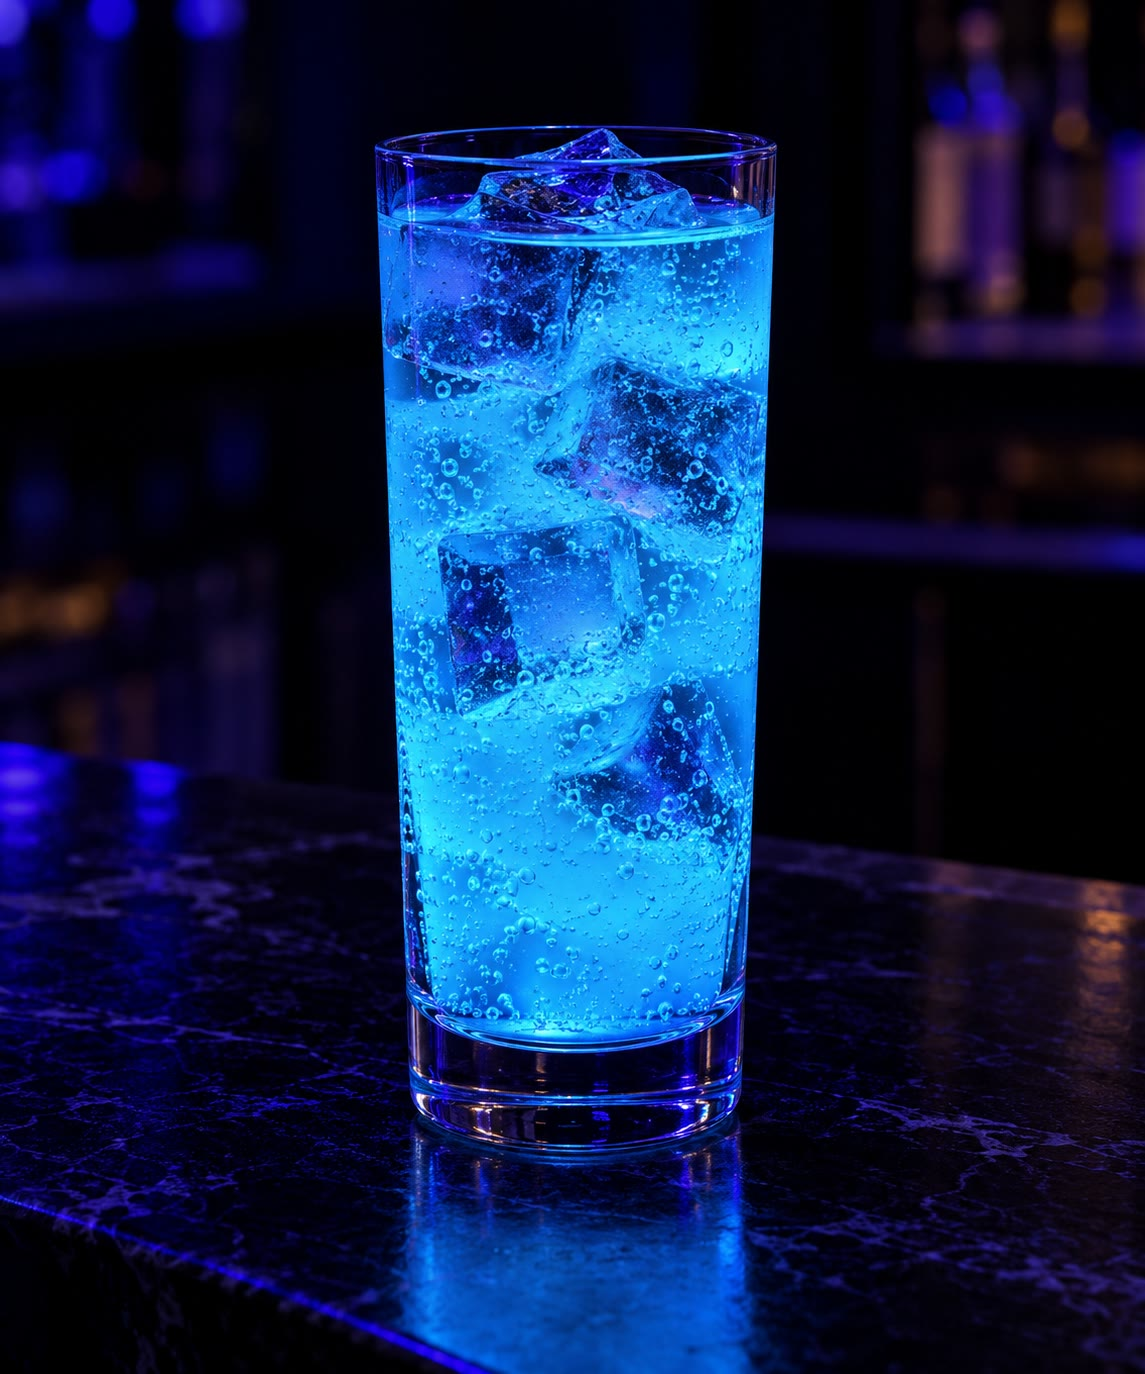
\includegraphics[height=4.6cm]{images/book4/ai/b3-07-tonic.jpg}\hspace{1em}%
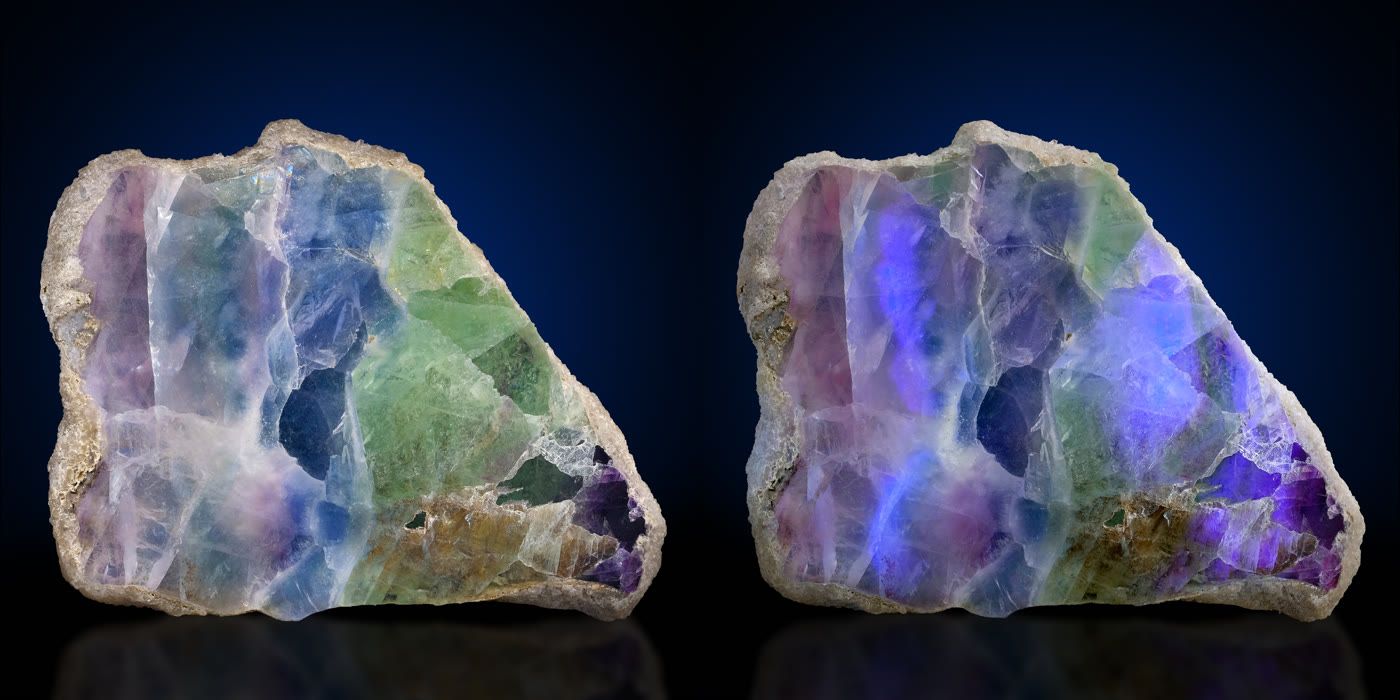
\includegraphics[height=4.6cm]{images/book4/fluorite-uv.jpg}

{\small À gauche~: du tonic luisant en bleu sous une lampe ultraviolette.
À droite~: de la fluorine à la lumière du jour et en \omterm{def:b3:electronic-spectroscopy:luminescence}{fluorescence} sous
ultraviolet~; c'est ce minéral qui a donné son nom à la \omterm{def:b3:electronic-spectroscopy:luminescence}{fluorescence}.
Photographie Masha Milshina, CC BY 4.0.}
\end{omfigure}

\section{Transitions électroniques et règles de sélection}

\begin{definition}[Moment dipolaire de transition, force d'oscillateur]\label{def:b3:electronic-spectroscopy:transition-dipole}
Le \emph{moment dipolaire de transition}\index{moment dipolaire de transition} entre
les états $\Psi_i$ et $\Psi_f$ est $\boldsymbol\mu_{fi} = \langle\Psi_f|\hat{\boldsymbol\mu}|\Psi_i
\rangle$, avec $\hat{\boldsymbol\mu} = -e\sum_k\mathbf r_k$ (plus les
charges nucléaires, dont les contributions s'annulent entre états
orthogonaux). La \emph{force
d'oscillateur}\index{force d'oscillateur} $f$ est la mesure sans dimension
de l'intensité d'une bande, voisine de 1 pour les transitions les plus
intenses.
\end{definition}

\begin{proposition}[Intensité et force d'oscillateur]\label{prop:b3:electronic-spectroscopy:intensity}
L'absorption intégrée d'une bande est proportionnelle à $|\boldsymbol\mu_{fi}|^2$,
et en pratique
\[
f \approx 4.32\times10^{-9}\int\varepsilon(\tilde\nu)\,\dd\tilde\nu,
\]
avec $\varepsilon$ en \unit{L.mol^{-1}.cm^{-1}} et $\tilde\nu$ en \unit{cm^{-1}}.
\end{proposition}
\admitted

La proportionnalité provient de la théorie des perturbations dépendant du
temps et le facteur numérique de l'oscillateur classique~; tous deux
relèvent de cours plus avancés. Ce qui compte ici est que $f$ n'est grand
que si
$\boldsymbol\mu_{fi}$ l'est, et que la symétrie peut l'annuler.

\begin{theorem}[La règle de sélection de spin]\label{thm:b3:electronic-spectroscopy:spin-rule}
Une transition dipolaire électrique entre états de spins totaux
différents est interdite~: $\Delta S = 0$.
\end{theorem}

\begin{proof}
Chaque état est le produit d'une fonction spatiale et d'une fonction de
spin, $\Psi = \phi\,\chi$.
L'\omterm{def:b3:quantum-model-systems:operator}{opérateur} dipolaire n'agit que sur les positions, donc $\langle\phi_f\chi_f|\hat{\boldsymbol\mu}|
\phi_i\chi_i\rangle = \langle\phi_f|\hat{\boldsymbol\mu}|\phi_i\rangle\langle\chi_f|\chi_i\rangle$.
Des fonctions de spin de $S$ différents sont \omterm{def:b3:quantum-model-systems:operator}{fonctions propres} de
$\hat S^2$ de \omterm{def:b3:quantum-model-systems:operator}{valeurs propres} différentes,
donc orthogonales (\cref{thm:b3:quantum-model-systems:hermitian-real})~:
le second facteur est nul.
\end{proof}

\begin{theorem}[La règle de Laporte]\label{thm:b3:electronic-spectroscopy:laporte}
Dans une molécule possédant un \omterm{def:b3:point-groups:inversion}{centre d'inversion}, une transition
dipolaire électrique doit changer la parité~: $g \leftrightarrow u$ est
permise, $g \leftrightarrow g$ et $u
\leftrightarrow u$ sont interdites. C'est la \emph{règle de Laporte}\index{regle de Laporte@règle de Laporte}.
\end{theorem}

\begin{proof}
Les composantes de $\hat{\boldsymbol\mu}$ changent de signe par
inversion~: elles sont $u$.
Le produit $\Gamma_f\otimes\Gamma_\mu\otimes\Gamma_i$ n'est $g$ que si
$\Gamma_f$ et $\Gamma_i$
sont de parités opposées~; sinon il est $u$ et ne peut pas contenir la
\omterm{def:b3:group-theory-applied:reducible}{représentation totalement symétrique}
(\cref{thm:b3:group-theory-applied:vanishing-integral}).
\end{proof}

Les deux règles sont strictes pour les états idéalisés~; les molécules
réelles les assouplissent --- le \omterm{def:b3:many-electron-atoms:spin-orbit}{couplage spin--orbite} mélange les
caractères singulet et triplet, les vibrations suppriment un instant le
centre de symétrie --- et les transitions «~interdites~» apparaissent,
faiblement. Les bandes $d$--$d$ des complexes octaédriques, interdites
par la \omterm{thm:b3:electronic-spectroscopy:laporte}{règle de Laporte} et faibles, doivent leur couleur à cet
assouplissement
(\cref{ch:b3:complex-spectra-magnetism}).

\begin{definition}[Transition de transfert de charge]\label{def:b3:electronic-spectroscopy:charge-transfer}
Une \emph{transition de transfert de charge}\index{transition de transfert de charge} fait passer
un électron d'une orbitale localisée principalement sur une partie d'un
système (un donneur) vers une orbitale localisée principalement sur une
autre (un accepteur)~; son moment de transition est grand, sa bande
intense et large, et son énergie sensible à la polarité du solvant.
\end{definition}

\begin{method}[Attribuer une bande d'absorption]\label{met:b3:electronic-spectroscopy:assign-band}
\begin{enumerate}
  \item $\varepsilon_{\max}$ supérieur à environ \qty{e4}{L.mol^{-1}.cm^{-1}}~:
        une transition permise ($\pi\to\pi^*$ d'un système conjugué, ou
        transfert de charge).
  \item $\varepsilon_{\max}$ de 10 à quelques centaines~: une transition
        interdite ($n\to\pi^*$,
        interdite par la symétrie~; $d$--$d$, interdite par la \omterm{thm:b3:electronic-spectroscopy:laporte}{règle de
        Laporte}).
  \item $\varepsilon_{\max}$ inférieur à 1~: interdite de spin.
  \item Une bande $n\to\pi^*$ se déplace vers les courtes longueurs
        d'onde dans les solvants protiques (le doublet non liant est
        stabilisé par les liaisons hydrogène), une bande $\pi\to\pi^*$
        en général vers les grandes.
\end{enumerate}
\end{method}

\section{Le principe de Franck--Condon}

\begin{theorem}[Principe de Franck--Condon]\label{thm:b3:electronic-spectroscopy:franck-condon}
Dans l'\omterm{def:b3:computational-chemistry:born-oppenheimer}{approximation de Born--Oppenheimer}, et si le moment de transition
dépend peu des positions des noyaux, l'intensité de la \omterm{def:b3:electronic-spectroscopy:vibronic}{transition
vibronique} du niveau de vibration $v''$ de l'état électronique inférieur
au niveau
$v'$ de l'état supérieur est proportionnelle à $|\langle\chi_{v'}|\chi_{v''}\rangle|^2$,
le carré du recouvrement des deux fonctions d'onde de vibration~: c'est
le \emph{principe de Franck--Condon}\index{principe de Franck--Condon}.
Les transitions électroniques sont verticales~: les noyaux ne bougent pas
pendant que les électrons sautent.
\end{theorem}

\begin{proof}
Avec $\Psi = \psi_{\mathrm{el}}(\mathbf r;R)\chi_v(R)$, le moment de transition vaut
$\int\chi_{v'}^*\big[\int\psi'^*_{\mathrm{el}}\hat\mu\psi''_{\mathrm{el}}\dd\mathbf r\big]
\chi_{v''}\,\dd R$. Le crochet est le moment de transition électronique
$\mu_{\mathrm{el}}(R)$~; pris constant (approximation de Condon), il sort
de l'intégrale, laissant $\mu_{\mathrm{el}}\langle\chi_{v'}|\chi_{v''}\rangle$.
\end{proof}

\begin{definition}[Transition vibronique, progression, facteur de Franck--Condon]\label{def:b3:electronic-spectroscopy:vibronic}
Une \emph{transition vibronique}\index{transition vibronique} change à la
fois l'état électronique et l'état de vibration~; les raies
$v' \leftarrow 0$ pour $v' = 0, 1, 2,
\dots$ forment une \emph{progression vibronique}\index{progression vibronique}~;
le \emph{facteur de Franck--Condon}\index{facteur de Franck--Condon} d'une
raie vibronique est
$|\langle\chi_{v'}|\chi_{v''}\rangle|^2$.
\end{definition}

\begin{proposition}[Oscillateurs décalés]\label{prop:b3:electronic-spectroscopy:displaced}
Si les deux états sont harmoniques, de même fréquence, et si le minimum
supérieur est décalé de $\Delta$ (en unités de $\sqrt{\hbar/m\omega}$),
les \omterm{def:b3:electronic-spectroscopy:vibronic}{facteurs de Franck--Condon} issus de $v'' = 0$ suivent une loi de
Poisson,
$|\langle v'|0\rangle|^2 = \eu^{-S}S^{v'}/v'!$, avec $S = \Delta^2/2$~; la
raie la plus intense se situe vers $v' = S$.
\end{proposition}
\admitted

La démonstration générale utilise les \omterm{def:b3:quantum-model-systems:ladder}{opérateurs d'échelle} du
\cref{ch:b3:quantum-model-systems}~; les données de figure de ce
chapitre confrontent la formule à une intégration directe. Un petit
décalage donne une seule raie 0--0 intense~; un grand décalage, une
longue progression dont le membre le plus intense est loin de la raie
0--0.

\begin{omfigure}
\begin{tikzpicture}
\begin{axis}[name=pc, width=0.46\linewidth, height=6cm, xmin=-4, xmax=5, ymin=0,
  ymax=14, axis lines=left, xtick=\empty, ytick=\empty, xlabel={coordonnée nucléaire},
  ylabel={énergie}, label style={font=\small}]
\addplot[black, thick] table[x=y, y=ground] {figdata/out/bachelor-3-franck-condon-curves.dat};
\addplot[omDef, thick] table[x=y, y=excited] {figdata/out/bachelor-3-franck-condon-curves.dat};
\draw[omabs] (axis cs:0,0.5) -- (axis cs:0,10.6);
\draw[omvib] (axis cs:-1,0.5) -- (axis cs:1,0.5);
\draw[omvib] (axis cs:0.732,9.5) -- (axis cs:2.732,9.5);
\draw[omvib] (axis cs:-0.000,10.5) -- (axis cs:3.464,10.5);
\draw[omvib] (axis cs:-0.504,11.5) -- (axis cs:3.968,11.5);
\draw[omvib] (axis cs:-0.914,12.5) -- (axis cs:4.378,12.5);
\node[font=\small, anchor=west] at (axis cs:-3.9,13.0) {excité};
\node[font=\small, anchor=east] at (axis cs:4.95,1.5) {fondamental};
\node[font=\scriptsize, anchor=east] at (axis cs:-0.05,5.5) {verticale};
\end{axis}
\begin{axis}[at={(pc.east)}, anchor=west, xshift=1.3cm, width=0.46\linewidth,
  height=6cm, xmin=-0.5, xmax=12.5, ymin=0, ymax=0.8, axis lines=left, ycomb,
  xlabel={$v'$}, ylabel={facteur de Franck--Condon}, label style={font=\small},
  tick label style={font=\small}]
\addplot[black, very thick] table[x=v, y=s03] {figdata/out/bachelor-3-franck-condon-sticks.dat};
\addplot[omDef, very thick, xshift=2pt] table[x=v, y=s15] {figdata/out/bachelor-3-franck-condon-sticks.dat};
\addplot[omThm, very thick, xshift=4pt] table[x=v, y=s5] {figdata/out/bachelor-3-franck-condon-sticks.dat};
\end{axis}
\end{tikzpicture}

{\small À gauche~: une transition verticale depuis le niveau le plus bas
de l'état fondamental aboutit là où la courbe excitée, décalée vers une
liaison plus longue, est bien au-dessus de son minimum (tracé pour
$S = 1.5$). À droite~: \omterm{def:b3:electronic-spectroscopy:vibronic}{facteurs de Franck--Condon} de la progression pour
$S = 0.3$ (noir), 1.5 (bleu) et 5 (rouge)~; chaque série a pour somme
1.}
\end{omfigure}

\begin{example}[Le diiode]\label{ex:b3:electronic-spectroscopy:iodine}
% ledger: diat:I2.re, diat:I2B.re, diat:I2B.we, imass:I127
La vapeur de diiode est violette parce que sa bande B$\leftarrow$X
absorbe la lumière jaune-vert.
La liaison s'allonge de \qty{266.6}{pm} dans l'état fondamental à
\qty{302.5}{pm} dans l'état B. Dans le modèle des oscillateurs décalés,
avec la fréquence de l'état B
(\qty{125.7}{cm^{-1}}), $\Delta R = \qty{35.8}{pm}$ donne $S \approx 15$~:
l'absorption est une longue progression dont les raies les plus intenses
aboutissent sur des niveaux de vibration élevés de l'état B, et dont le
prolongement se fond dans le continuum de dissociation.
\end{example}

\section{Le devenir d'un état excité~: le diagramme de Jablonski}

\begin{definition}[Diagramme de Jablonski]\label{def:b3:electronic-spectroscopy:jablonski}
Un \emph{diagramme de Jablonski}\index{diagramme de Jablonski} représente
les états électroniques d'une molécule (singulets $S_0, S_1, S_2, \dots$
dans une colonne, triplets $T_1, T_2,
\dots$ dans une autre), leurs niveaux de vibration, et les processus qui
les relient~: les processus radiatifs par des flèches droites, les
processus non radiatifs par des flèches ondulées.
\end{definition}

\begin{definition}[Processus non radiatifs]\label{def:b3:electronic-spectroscopy:radiationless}
La \emph{relaxation vibrationnelle}\index{relaxation vibrationnelle} amène
une molécule excitée au niveau de vibration le plus bas de son état
électronique par collisions, en quelques picosecondes. La
\emph{conversion interne}\index{conversion interne}
est une transition non radiative entre états de même
multiplicité ($S_2 \to S_1$, $S_1 \to S_0$)~; le \emph{croisement
intersystème}\index{croisement intersysteme@croisement intersystème}, une
transition non radiative entre états de multiplicités différentes
($S_1 \to T_1$, $T_1 \to S_0$).
\end{definition}

\begin{definition}[Luminescence, fluorescence, phosphorescence, déplacement de Stokes]\label{def:b3:electronic-spectroscopy:luminescence}
La \emph{luminescence}\index{luminescence} est l'émission de lumière par
une molécule excitée. La \emph{fluorescence}\index{fluorescence} est une
émission permise de spin,
en général $S_1 \to S_0$, rapide (nanosecondes)~; la \emph{phosphorescence}\index{phosphorescence}
est une émission interdite de spin, en général $T_1 \to S_0$, lente
(millisecondes à secondes). Le \emph{déplacement de Stokes}\index{deplacement de Stokes@déplacement de Stokes} est
l'écart entre les maxima d'absorption et d'émission, exprimé en énergie.
\end{definition}

\begin{omfigure}
\begin{tikzpicture}[font=\small, >=Stealth]
  \foreach \y/\l in {0/{$S_0$}, 3.4/{$S_1$}, 5.6/{$S_2$}}{
    \draw[omstate] (0,\y) -- (3.6,\y); \node[anchor=east] at (-0.1,\y) {\l};
    \foreach \d in {0.25,0.5,0.75}{\draw[omvib] (0,\y+\d) -- (3.6,\y+\d);}}
  \draw[omstate] (5.0,2.5) -- (7.6,2.5); \node[anchor=west] at (7.7,2.5) {$T_1$};
  \foreach \d in {0.25,0.5,0.75}{\draw[omvib] (5.0,2.5+\d) -- (7.6,2.5+\d);}
  \draw[omabs] (0.3,0) -- (0.3,4.15) node[pos=0.35, left, font=\scriptsize, align=right] {absorption};
  \draw[omabs] (0.7,0) -- (0.7,5.85);
  \draw[omnonrad] (1.05,5.85) -- (1.05,5.6);
  \draw[omnonrad] (1.05,5.6) -- (1.05,3.4) node[pos=0.5, right, font=\scriptsize] {IC};
  \draw[omnonrad] (0.45,4.15) -- (0.45,3.42);
  \draw[omfluo] (1.7,3.4) -- (1.7,0.5) node[pos=0.5, right, font=\scriptsize, align=left] {fluor-\\escence};
  \draw[omnonrad] (3.2,3.4) -- (3.2,0.02) node[pos=0.5, right, font=\scriptsize] {IC};
  \draw[omisc] (3.6,3.4) -- (5.0,3.1) node[pos=0.5, above, font=\scriptsize] {ISC};
  \draw[omnonrad] (5.3,3.1) -- (5.3,2.52);
  \draw[omphos] (6.0,2.5) -- (6.0,0.5) node[pos=0.5, right, font=\scriptsize, align=left] {phosphor-\\escence};
  \draw[omisc] (5.6,2.5) -- (3.7,0.02) node[pos=0.45, above left, font=\scriptsize, inner sep=1pt] {ISC};
  \draw[omvib, dashed] (3.6,0.5) -- (6.0,0.5);
  \draw[omvib, dashed] (3.6,0.0) -- (7.6,0.0);
\end{tikzpicture}

{\small Un \omterm{def:b3:electronic-spectroscopy:jablonski}{diagramme de Jablonski}. Flèches droites~: absorption (bleu),
\omterm{def:b3:electronic-spectroscopy:luminescence}{fluorescence} (rouge), \omterm{def:b3:electronic-spectroscopy:luminescence}{phosphorescence} (orange)~; flèches ondulées~:
\omterm{def:b3:electronic-spectroscopy:radiationless}{relaxation vibrationnelle} et \omterm{def:b3:electronic-spectroscopy:radiationless}{conversion interne} (IC)~; flèches ondulées
en tirets~: \omterm{def:b3:electronic-spectroscopy:radiationless}{croisement intersystème} (ISC).
L'émission part du niveau de vibration le plus bas de $S_1$ ou de $T_1$
et peut aboutir sur n'importe quel niveau de $S_0$.}
\end{omfigure}

\begin{proposition}[Règle de Kasha]\label{prop:b3:electronic-spectroscopy:kasha}
La \omterm{def:b3:electronic-spectroscopy:luminescence}{luminescence} se produit, à de très rares exceptions près, depuis
l'état excité le plus bas d'une multiplicité donnée ($S_1$ ou $T_1$),
quel que soit l'état excité initialement~: c'est la
\emph{règle de Kasha}\index{regle de Kasha@règle de Kasha}.
\end{proposition}
\begin{proof}[Statut]
Établie expérimentalement~; la raison en est que la \omterm{def:b3:electronic-spectroscopy:radiationless}{conversion interne}
entre états excités supérieurs, proches les uns des autres, est bien plus
rapide que l'émission, alors que l'écart $S_1$--$S_0$ est grand.
\end{proof}

\begin{proposition}[Image miroir]\label{prop:b3:electronic-spectroscopy:mirror}
Si les états excité et fondamental ont des structures de vibration
semblables, la bande de \omterm{def:b3:electronic-spectroscopy:luminescence}{fluorescence} est l'image miroir de la première
bande d'absorption par rapport à leur raie 0--0 commune~; l'émission se
situe à plus grande longueur d'onde (\omterm{def:b3:electronic-spectroscopy:luminescence}{déplacement de Stokes}).
\end{proposition}

\begin{proof}
L'absorption va de $v'' = 0$ aux niveaux $v'$ de $S_1$, à $E_{00} + v'h\nu'$~;
l'émission va de $v' = 0$ aux niveaux $v''$ de $S_0$, à $E_{00} - v''h\nu''$.
Avec des fréquences égales et les mêmes \omterm{def:b3:electronic-spectroscopy:vibronic}{facteurs de Franck--Condon} (même
décalage), les deux progressions sont symétriques par rapport à
$E_{00}$.
\end{proof}

\begin{omfigure}
\begin{tikzpicture}
\begin{axis}[width=0.75\linewidth, height=5cm, xmin=17, xmax=33, ymin=0,
  ymax=1.15, axis x line=bottom, axis y line=left, ytick=\empty,
  xlabel={nombre d'onde / $10^3$ cm$^{-1}$}, ylabel={intensité},
  legend cell align=left, legend style={font=\small, draw=none, at={(0.02,0.97)}, anchor=north west},
  tick label style={font=\small}, label style={font=\small}]
\addplot[omDef, thick] table[x=nu, y=abs] {figdata/out/bachelor-3-photophysics-bands.dat};
\addlegendentry{absorption}
\addplot[omThm, thick] table[x=nu, y=em] {figdata/out/bachelor-3-photophysics-bands.dat};
\addlegendentry{fluorescence}
\draw[gray, dashed] (axis cs:25,0) -- (axis cs:25,1.12);
\node[font=\scriptsize, gray, anchor=south west] at (axis cs:25,1.0) {0--0};
\end{axis}
\end{tikzpicture}

{\small Absorption et \omterm{def:b3:electronic-spectroscopy:luminescence}{fluorescence} d'une molécule modèle ($S = 1$,
quantum de vibration de \qty{1400}{cm^{-1}})~: images miroirs par
rapport à la raie 0--0~; les maxima sont séparés par le \omterm{def:b3:electronic-spectroscopy:luminescence}{déplacement de
Stokes}.}
\end{omfigure}

\section{Cinétique des états excités}

Après l'excitation, la population de $S_1$ décroît par tous les processus
qui lui sont ouverts, chacun d'ordre 1~: désexcitation radiative $k_r$,
\omterm{def:b3:electronic-spectroscopy:radiationless}{conversion interne} $k_{\mathrm{IC}}$,
\omterm{def:b3:electronic-spectroscopy:radiationless}{croisement intersystème} $k_{\mathrm{ISC}}$.

\begin{definition}[Durée de vie de l'état excité, durée de vie radiative]\label{def:b3:electronic-spectroscopy:lifetime}
La \emph{durée de vie de l'état excité}\index{duree de vie de l'etat excite@durée de vie de l'état excité} est $\tau =
1/\sum k$, la constante de temps de la décroissance exponentielle de la
population excitée. La \emph{durée de vie radiative}\index{duree de vie radiative@durée de vie radiative} $\tau_r =
1/k_r$ est la durée de vie qu'aurait l'état si l'émission était son seul
devenir.
\end{definition}

\begin{definition}[Rendement quantique]\label{def:b3:electronic-spectroscopy:quantum-yield}
Le \emph{rendement quantique}\index{rendement quantique} d'un processus
consécutif à l'absorption de lumière est le nombre d'événements de ce
processus divisé par le nombre de photons absorbés. Le \emph{rendement
quantique de fluorescence}\index{rendement quantique de fluorescence} $\Phi_F$ est le
nombre de photons émis par \omterm{def:b3:electronic-spectroscopy:luminescence}{fluorescence} par photon absorbé.
\end{definition}

\begin{proposition}[Rendement quantique et durée de vie]\label{prop:b3:electronic-spectroscopy:quantum-yield}
$\Phi_F = k_r/(k_r + k_{\mathrm{IC}} + k_{\mathrm{ISC}}) = k_r\tau = \tau/\tau_r$~; de même,
$\Phi_{\mathrm{ISC}} = k_{\mathrm{ISC}}\tau$, et les rendements des
processus en compétition ont pour somme 1.
\end{proposition}

\begin{proof}
$\dd[S_1]/\dd t = -(k_r + k_{\mathrm{IC}} + k_{\mathrm{ISC}})[S_1]$, donc $[S_1] = [S_1]_0\eu^{-t/\tau}$.
Le nombre de photons émis est $\int_0^\infty k_r[S_1]\,\dd t = k_r\tau[S_1]_0$, sur
$[S_1]_0$ molécules excitées. La même intégrale avec chaque $k$ donne
chaque rendement, et leur somme vaut $\tau\sum k = 1$.
\end{proof}

\begin{definition}[Inhibiteur de fluorescence, inhibition dynamique et statique]\label{def:b3:electronic-spectroscopy:quencher}
Un \emph{inhibiteur de fluorescence}\index{inhibiteur de fluorescence} est
une espèce qui diminue la \omterm{def:b3:electronic-spectroscopy:luminescence}{fluorescence}. Dans l'\emph{inhibition
dynamique}\index{inhibition dynamique}, il désactive la molécule excitée
lors d'une collision, ajoutant une vitesse $k_q[Q]$ et raccourcissant la
durée de vie~; dans l'\emph{inhibition statique}\index{inhibition statique},
il forme un complexe non fluorescent avec la molécule dans son état
fondamental, ce qui diminue l'intensité sans changer la durée de vie des
molécules qui émettent encore.
\end{definition}

\begin{theorem}[Équation de Stern--Volmer]\label{thm:b3:electronic-spectroscopy:stern-volmer}
Pour une \omterm{def:b3:electronic-spectroscopy:quencher}{inhibition dynamique},
\[
\frac{I_0}{I} = \frac{\tau_0}{\tau} = 1 + k_q\tau_0[Q] = 1 + K_{SV}[Q],
\]
c'est l'\emph{équation de Stern--Volmer}\index{equation de Stern--Volmer@équation de Stern--Volmer}, où $I_0$ et $\tau_0$
sont mesurés sans inhibiteur et $K_{SV} = k_q\tau_0$.
\end{theorem}

\begin{proof}
Avec l'inhibiteur, $\tau = 1/(k_0 + k_q[Q])$ avec $k_0 = 1/\tau_0$, donc $\tau_0/\tau = 1 +
k_q\tau_0[Q]$. L'intensité est proportionnelle à $\Phi_F = k_r\tau$, donc $I_0/I = \tau_0/\tau$.
\end{proof}

\begin{omfigure}
\begin{tikzpicture}
\begin{axis}[name=dec, width=0.5\linewidth, height=5cm, xmin=0, xmax=40, ymode=log,
  ymin=0.005, ymax=1.2, axis lines=left, xlabel={$t$ / ns}, ylabel={$I(t)/I(0)$},
  legend cell align=left, legend style={font=\scriptsize, draw=none, at={(0.98,0.98)}, anchor=north east},
  tick label style={font=\small}, label style={font=\small}]
\addplot[black, thick] table[x=t, y=q0] {figdata/out/bachelor-3-photophysics-decays.dat};
\addlegendentry{$[Q] = 0$}
\addplot[omDef, thick] table[x=t, y=q1] {figdata/out/bachelor-3-photophysics-decays.dat};
\addlegendentry{0.01 M}
\addplot[omProp, thick] table[x=t, y=q2] {figdata/out/bachelor-3-photophysics-decays.dat};
\addlegendentry{0.02 M}
\addplot[omThm, thick] table[x=t, y=q4] {figdata/out/bachelor-3-photophysics-decays.dat};
\addlegendentry{0.04 M}
\end{axis}
\begin{axis}[at={(dec.east)}, anchor=west, xshift=1.4cm, width=0.42\linewidth,
  height=5cm, xmin=0, xmax=0.045, ymin=0, ymax=3.3, axis lines=left,
  xlabel={$[Q]$ / mol L$^{-1}$}, ylabel={$I_0/I = \tau_0/\tau$},
  xticklabel style={/pgf/number format/fixed, /pgf/number format/precision=2},
  scaled x ticks=false, tick label style={font=\small}, label style={font=\small}]
\addplot[omThm, thick, mark=*] table[x=Q, y=I0I] {figdata/out/bachelor-3-photophysics-sv.dat};
\end{axis}
\end{tikzpicture}

{\small \omterm{def:b3:electronic-spectroscopy:quencher}{Inhibition dynamique} d'un fluorophore modèle ($\tau_0 = \qty{10}{ns}$, $k_q =
\qty{5e9}{L.mol^{-1}.s^{-1}}$). À gauche~: déclins de \omterm{def:b3:electronic-spectroscopy:luminescence}{fluorescence},
droites en échelle logarithmique, d'autant plus raides que l'inhibiteur
est abondant. À droite~: la droite de Stern--Volmer, de pente
$K_{SV} = k_q\tau_0 = \qty{50}{L/mol}$.}
\end{omfigure}

\begin{method}[Rendement quantique de fluorescence relatif]\label{met:b3:electronic-spectroscopy:relative-yield}
\begin{enumerate}
  \item Choisir un étalon de $\Phi_{\mathrm{std}}$ connu absorbant à la
        même longueur d'onde d'excitation.
  \item Préparer des solutions diluées ($A < 0.1$, pour éviter la
        réabsorption) et enregistrer leurs absorbances $A$ et leurs
        spectres d'émission intégrés $F$ dans des conditions identiques.
  \item $\Phi = \Phi_{\mathrm{std}}\,\dfrac{F}{F_{\mathrm{std}}}\,\dfrac{A_{\mathrm{std}}}{A}\,
        \dfrac{n^2}{n_{\mathrm{std}}^2}$, le dernier facteur corrigeant
        l'effet des indices de réfraction des solvants.
\end{enumerate}
\end{method}

\begin{method}[Analyser des données d'inhibition]\label{met:b3:electronic-spectroscopy:stern-volmer}
\begin{enumerate}
  \item Tracer $I_0/I$ en fonction de $[Q]$~; une droite passant par 1
        donne $K_{SV}$.
  \item Mesurer aussi les durées de vie~: si $\tau_0/\tau$ suit la même
        droite, l'inhibition
        est dynamique, et $k_q = K_{SV}/\tau_0$~; si $\tau$ ne change pas,
        elle est statique.
  \item Comparer $k_q$ à la limite de diffusion, environ
        \qty{e10}{L.mol^{-1}.s^{-1}} dans
        l'eau (\cref{ch:b3:rate-theories})~: un $k_q$ qui en est proche
        signifie que presque chaque rencontre désactive.
\end{enumerate}
\end{method}

\begin{example}[Quinine et anthracène]\label{ex:b3:electronic-spectroscopy:quinine}
% ledger: fl:quinine.labs, fl:quinine.eps, fl:quinine.phi, fl:anthracene.labs, fl:anthracene.phi
Le sulfate de quinine dans l'acide sulfurique à \qty{0.5}{M} absorbe à
\qty{349}{nm} avec $\varepsilon =
\qty{5700}{L.mol^{-1}.cm^{-1}}$ et fluoresce avec $\Phi_F = 0.546$, ce qui
en fait l'étalon classique des \omterm{def:b3:electronic-spectroscopy:quantum-yield}{rendements quantiques} relatifs.
L'anthracène dans le cyclohexane
absorbe à \qty{356}{nm} et a $\Phi_F = 0.36$~; l'essentiel du reste de
ses molécules excitées passe au triplet.
\end{example}

\section{Applications}

La \omterm{def:b3:electronic-spectroscopy:luminescence}{fluorescence} se détecte sur un fond noir, ce qui rend la fluorimétrie
cent à mille fois plus sensible que la spectroscopie d'absorption~: on
mesure couramment des concentrations nanomolaires d'un composé
fluorescent. Les sondes fluorescentes renseignent sur leur environnement
par leur longueur d'onde, leur rendement ou leur durée de vie (polarité,
pH, fixation d'un ion)~; le transfert d'énergie entre deux fluorophores,
efficace seulement sur quelques nanomètres, mesure des distances dans
les protéines. Les complexes phosphorescents de métaux lourds, dans
lesquels le \omterm{def:b3:many-electron-atoms:spin-orbit}{couplage spin--orbite} rend le \omterm{def:b3:electronic-spectroscopy:radiationless}{croisement intersystème}
efficace, récoltent les triplets dans les diodes électroluminescentes
des écrans.

\begin{inthelab}[Comptage de photons uniques corrélé en temps]
Pour mesurer une durée de vie de l'ordre de la nanoseconde, on excite
l'échantillon par une diode laser pulsée à une cadence de l'ordre du
mégahertz, et l'on enregistre pour chaque impulsion le retard du premier
photon de \omterm{def:b3:electronic-spectroscopy:luminescence}{fluorescence} détecté. Après des millions d'impulsions,
l'histogramme des retards est la courbe de déclin, sur laquelle on ajuste
$\tau$, la réponse de l'instrument étant mesurée sur une solution
diffusante. La source ultraviolette est capotée~; l'opérateur porte des
lunettes qui arrêtent sa longueur d'onde.
\end{inthelab}

\begin{history}[Stokes, 1852]
George Gabriel Stokes fit passer la lumière du Soleil à travers un verre
violet et un prisme jusqu'à une solution de quinine, et vit une lumière
bleue émerger de la région éclairée par les rayons ultraviolets
invisibles~: la lumière émise avait toujours une longueur d'onde plus
grande que la lumière absorbée. Il appela ce phénomène \omterm{def:b3:electronic-spectroscopy:luminescence}{fluorescence},
d'après la fluorine, un minéral qui luit de la même façon.
\end{history}

\section{Exercices}

\begin{exercise}[$\star$]\label{exo:b3:electronic-spectroscopy:1}
Permise ou interdite, et selon quelle règle~: (a) $S_0 \to T_1$ dans le
benzène~; (b) une transition $d$--$d$ d'un complexe octaédrique~; (c) la
transition $\pi\to\pi^*$ de l'éthène
($B_{1u} \leftarrow A_g$ dans $D_{2h}$)~; (d) la transition $n\to\pi^*$
du méthanal
($A_2$)~?
\end{exercise}

\begin{exercise}[$\star$]\label{exo:b3:electronic-spectroscopy:2}
Un composé absorbe à \qty{349}{nm} et fluoresce avec un maximum à
\qty{450}{nm} (données de l'exercice). Calculer le \omterm{def:b3:electronic-spectroscopy:luminescence}{déplacement de Stokes}
en \unit{cm^{-1}} et en
eV.
\end{exercise}

\begin{exercise}[$\star$]\label{exo:b3:electronic-spectroscopy:3}
% ledger: fl:quinine.eps
Calculer l'absorbance à \qty{349}{nm} d'une solution de sulfate de
quinine à \qty{1.0e-5}{mol/L} dans une cuve de \qty{1}{cm}, et la
fraction de la lumière qu'elle absorbe.
\end{exercise}

\begin{exercise}[$\star$]\label{exo:b3:electronic-spectroscopy:4}
Un fluorophore a $\Phi_F = 0.60$ et $\tau = \qty{4.0}{ns}$. Calculer $k_r$,
la \omterm{def:b3:electronic-spectroscopy:lifetime}{durée de vie radiative} et la somme des constantes de vitesse non
radiatives.
\end{exercise}

\begin{exercise}[$\star\star$]\label{exo:b3:electronic-spectroscopy:5}
Une bande est gaussienne, avec $\varepsilon_{\max} = \qty{5700}{L.mol^{-1}.cm^{-1}}$ et une largeur à
mi-hauteur de \qty{5000}{cm^{-1}}. Estimer sa \omterm{def:b3:electronic-spectroscopy:transition-dipole}{force d'oscillateur}
(l'intégrale d'une gaussienne vaut $1.0645\,\varepsilon_{\max}\times$la
largeur à mi-hauteur).
\end{exercise}

\begin{exercise}[$\star\star$]\label{exo:b3:electronic-spectroscopy:6}
Pour des oscillateurs décalés, trouver la raie la plus intense de la
progression pour
$S = 0.3$, 1.5 et 5, et le rapport de son facteur à celui de la raie
0--0.
\end{exercise}

\begin{exercise}[$\star\star$]\label{exo:b3:electronic-spectroscopy:7}
Depuis $S_1$, $k_r = \qty{1.0e8}{s^{-1}}$, $k_{\mathrm{IC}} = \qty{2.0e7}{s^{-1}}$ et $k_{\mathrm{ISC}} =
\qty{3.0e8}{s^{-1}}$. Calculer $\tau$, $\Phi_F$ et $\Phi_{\mathrm{ISC}}$.
\end{exercise}

\begin{exercise}[$\star\star$]\label{exo:b3:electronic-spectroscopy:8}
% ledger: fl:quinine.phi, nD:water, nD:cyclohexane
La \omterm{def:b3:electronic-spectroscopy:luminescence}{fluorescence} de l'anthracène dans le cyclohexane ($A = 0.040$) a une
intégrale égale à 0.46 fois celle du sulfate de quinine dans l'acide
sulfurique dilué ($A = 0.050$, $\Phi =
0.546$). Avec les indices de réfraction 1.4266 (cyclohexane) et 1.333
(eau, pour l'acide dilué), calculer $\Phi_F$ de l'anthracène.
\end{exercise}

\begin{exercise}[$\star\star$]\label{exo:b3:electronic-spectroscopy:9}
La durée de vie d'un fluorophore vaut 8.0, 5.6 et \qty{4.3}{ns} pour des
concentrations d'inhibiteur de 0, 0.010 et \qty{0.020}{mol/L}.
L'inhibition est-elle dynamique~? Trouver
$K_{SV}$ et $k_q$.
\end{exercise}

\begin{exercise}[$\star\star\star$]\label{exo:b3:electronic-spectroscopy:10}
L'ajout d'un inhibiteur divise par deux l'intensité de \omterm{def:b3:electronic-spectroscopy:luminescence}{fluorescence} alors
que la durée de vie mesurée reste de \qty{6.0}{ns}. De quel type
d'inhibition s'agit-il, et qu'implique-t-elle pour l'état fondamental~?
Écrire la relation correspondante entre $I_0/I$
et la constante d'association du complexe.
\end{exercise}

\begin{exercise}[$\star\star\star$]\label{exo:b3:electronic-spectroscopy:11}
% ledger: fl:anthracene.phi
L'anthracène dans le cyclohexane a $\Phi_F = 0.36$ et, dans les
conditions d'une mesure, $\tau = \qty{5.0}{ns}$ (données de l'exercice).
Calculer $\tau_r$, ainsi que le rendement du triplet si la \omterm{def:b3:electronic-spectroscopy:radiationless}{conversion
interne} est négligeable. Pourquoi la \omterm{def:b3:electronic-spectroscopy:lifetime}{durée de vie radiative} est-elle plus
longue que la durée de vie mesurée~?
\end{exercise}

\begin{exercise}[$\star\star\star$]\label{exo:b3:electronic-spectroscopy:12}
Pour deux électrons, la fonction de spin singulet est $\frac{1}{\sqrt2}[\alpha\beta - \beta\alpha]$
et la fonction triplet $M_S = 0$ est $\frac{1}{\sqrt2}[\alpha\beta + \beta\alpha]$.
Montrer qu'elles sont orthogonales, et conclure sur l'intensité de
$T_1 \leftarrow S_0$ en l'absence de \omterm{def:b3:many-electron-atoms:spin-orbit}{couplage spin--orbite}.
\end{exercise}

\section{Problème~: pourquoi le tonic luit}

\begin{problem}[{Problème du week-end --- l'absorption par la quinine, le
devenir de son état excité, l'inhibition par les ions chlorure, et la
question de savoir si chaque rencontre désactive}]
\label{pb:b3:electronic-spectroscopy:1}
% ledger: fl:quinine.labs, fl:quinine.eps, fl:quinine.phi, visc:H2O.25C
Sulfate de quinine dans l'acide sulfurique à \qty{0.5}{M}~: maximum
d'absorption à \qty{349}{nm},
$\varepsilon = \qty{5700}{L.mol^{-1}.cm^{-1}}$, $\Phi_F = 0.546$. Données
du problème~: la durée de vie de \omterm{def:b3:electronic-spectroscopy:luminescence}{fluorescence} sans inhibiteur vaut
$\tau_0 = \qty{19}{ns}$~; le maximum d'émission est voisin de
\qty{450}{nm}~; l'ajout de chlorure de sodium donne les rapports
d'intensité
\begin{center}\small
\begin{tabular}{lccccc}
\hline
$[\ce{Cl-}]$ / mol L$^{-1}$ & 0 & 0.010 & 0.020 & 0.040 & 0.080 \\
$I_0/I$ & 1.000 & 1.594 & 2.188 & 3.376 & 5.752 \\ \hline
\end{tabular}
\end{center}
L'eau à \qty{25}{\celsius} a une viscosité de \qty{0.890}{mPa.s}~; $R =
\qty{8.314}{J.K^{-1}.mol^{-1}}$.

\medskip\noindent\textbf{Partie I --- L'absorption.}
\begin{enumerate}
  \item Calculer l'absorbance à \qty{349}{nm} d'une solution à
        \qty{1.0e-4}{mol/L} dans une cuve de
        \qty{1}{cm}.
  \item Quelle fraction de la lumière incidente est absorbée~?
  \item La transition est-elle permise~? Utiliser $\varepsilon$.
  \item Donner l'énergie du photon absorbé en eV.
  \item Pourquoi l'œil ne voit-il aucune couleur d'absorption dans le
        tonic~?
  \item Pourquoi maintient-on une solution destinée à la \omterm{def:b3:electronic-spectroscopy:luminescence}{fluorescence}
        au-dessous de $A = 0.1$~?
\end{enumerate}

\medskip\noindent\textbf{Partie II --- L'état excité.}
\begin{enumerate}[resume]
  \item Dessiner le \omterm{def:b3:electronic-spectroscopy:jablonski}{diagramme de Jablonski} des processus issus de $S_1$.
  \item Calculer la constante de vitesse radiative $k_r$ et la \omterm{def:b3:electronic-spectroscopy:lifetime}{durée de
        vie radiative}.
  \item Calculer la constante de vitesse non radiative totale.
  \item Calculer le \omterm{def:b3:electronic-spectroscopy:luminescence}{déplacement de Stokes} en \unit{cm^{-1}}.
  \item Pourquoi l'émission est-elle bleue alors que l'absorption se
        situe dans l'ultraviolet~?
  \item Quelle fraction de l'énergie absorbée repart sous forme de
        \omterm{def:b3:electronic-spectroscopy:luminescence}{fluorescence}, compte tenu de l'énergie de chaque photon~?
\end{enumerate}

\medskip\noindent\textbf{Partie III --- L'inhibition par le chlorure.}
\begin{enumerate}[resume]
  \item Tracer $I_0/I$ en fonction de $[\ce{Cl-}]$ et vérifier que la
        courbe est une droite.
  \item Déterminer $K_{SV}$ par les moindres carrés sur les cinq points.
  \item En supposant l'\omterm{def:b3:electronic-spectroscopy:quencher}{inhibition dynamique}, calculer $k_q$.
  \item Quelle durée de vie mesurerait-on à \qty{0.040}{mol/L}~?
  \item Comment prouver expérimentalement que l'inhibition est
        dynamique~?
  \item Pourquoi le tonic, qui ne contient pas de chlorure, est-il un bon
        milieu pour que la quinine luise~?
\end{enumerate}

\medskip\noindent\textbf{Partie IV --- Chaque rencontre~?}
\begin{enumerate}[resume]
  \item La constante de vitesse des rencontres contrôlées par la diffusion
        dans un solvant de viscosité $\eta$ vaut $k_d \approx 8RT/3\eta$.
        La calculer en \unit{L.mol^{-1}.s^{-1}}.
  \item Comparer $k_q$ et $k_d$.
  \item Quelle fraction des rencontres conduit à une désactivation~?
  \item L'inhibition serait-elle plus rapide ou plus lente dans un
        solvant plus visqueux~?
  \item Énoncer le résultat~: le rapport $k_q/k_d$ pour l'inhibition de
        la quinine par le chlorure.
\end{enumerate}
\end{problem}
